\section{Introduction}
In the first part of this report we want to present the physical concepts needed for the understanding of the performed calculations. At the end, the Split-Step Fourier method, which we used to analyze the dynamics of the different quantum systems, is introduced. \\

The Gross-Pitaevskii equation (GPE) successfully describes the dynamics of Bose-Einstein condensates. Here, we want to introduce the corresponding physical situation, along with its assumptions.

\subsection{Bose-Einstein condensation}

Bose-Einstein condensates (BECs) are states of matter of dilute boson gases cooled down to temperatures very close to absolute zero.

The most important characteristic of such system is, that a large fraction of bosons occupies the lowest quantum state.
Although one would assume that the understanding of the dynamics of a BEC is based on the microscopic, i.e. the quantum-mechanical, properties of the single bosons forming the gas, it is possible to describe Bose-Einstein condensates with one single, macroscopic wave function $\psi(\mathbf{r},t)$.

For an exact description of $N$ interacting quantum particles we would need the $N$-body wavefunction, $\psi(r_1, r_2, ...r_N , t)$, which obeys the many-body Schr\"odinger equation.
We assume the interactions between the particles to be very weak, which is well-founded in the diluteness of the gases and the weak forces between neutral atoms. 
By neglecting the effects of quantum fluctuations, the many-body wave function for large particle numbers ($N \gg 1$) is replaced by an \textit{effective} single-particle wave function $\psi_{\text{eff}}(\mathbf{r},t).$ 

In a field-theoretical approach to the subject, one would introduce this macroscopical wave function as a complex field of the form
\begin{align}
	\psi_{\text{eff}}(\mathbf{r},t) = \sqrt{n} \cdot \exp(\frac{i}{\hbar} \ \mathcal{S}(\mathbf{r},t))\label{eqn:Field equation}
\end{align}
 with the density and phase distributions $n$ and $\mathcal{S}$ of the condensate. It is normalized to the particle number $N$, such that
 \begin{align}
 	\int \dd[3]\mathbf{r} \ \norm{\psi}^2 = N.
 \end{align}

\subsection{From the Schr\"odinger equation to the GPE}
For an ideal Bose gas, i.\,e. without interactions between the particles, the evolution of the system over time would be governed by the time-dependent Schr\"odinger equation

\begin{align}
i\hbar\ \frac{\partial\psi(\mathbf{r}, t)}{\partial t} =
\left[ -\frac{\hbar^2}{2m} \nabla^2 + V(\mathbf{r}, t)\right]\psi(\mathbf{r}, t) \label{eqn:Schroedinger}
\end{align}

with the Laplacian $\nabla^2$ and the potential 
$V(\mathbf{r},t)$. 

One needs to modify this equation to include the particle interactions to describe the physical situation more precisely. We assume that elastic next-neighbor interactions between two single particles due to Van-der-Waals forces dominate the interaction processes inside the gas. This allows us to describe these processes using the model of hard-sphere interactions, which yields
\begin{align}
	\mathcal{U}(\mathbf{r_1}, \mathbf{r_2}) = g_{\tiny3D}\cdot \delta_D(\mathbf{r_1} - \mathbf{r_2})
\end{align}

for the interaction potential, where the interaction strength $g_{3D}$ is defined as
\begin{align}
	g_{\tiny{3D}} = \frac{4\pi\hbar^2 a_s}{m}
\end{align}
 with the scattering length $a_s$ in the low-energy limit. 

 Taking these interactions into accounts yields us to the modified, nonlinear version of the Schr\"odinger equation, the \textit{Gross-Pitaevskii equation}
\begin{align}
	i\hbar \ \frac{\partial\psi(\mathbf{r}, t)}{\partial t} = \left[-\frac{\hbar^2}{2m}\nabla^2 + V(\mathbf{r}, t) + g\norm{\psi}^2\right]\psi(\mathbf{r}, t).
\end{align}
All numerical calculations in this project are based on this equation. \\

\textbf{Some words on the Bogoliubov mean-field approach:} Working with field operators $\hat{\psi}$, induced by equation (\ref{eqn:Field equation}) leads us to a Hamiltonian description of the situation with the grand canonical Hamiltonian, here in one spatial dimension
\begin{align}
	\hat{\mathcal{H}} = \int \dd z \ \hat{\psi}^{\dagger}(z) \left[ -\frac{\hbar^2}{2m}\partial_z^2 + V(z) - \mu + \frac{g_{1D}}{2}\hat{\psi}^{\dagger}(z)\hat{\psi}(z)\right]\hat{\psi}(z)
\end{align}
where $g_{1D}$ is the interaction parameter for one dimension and $\mu$ is the chemical potential.

Choosing suitable parameters for the spatial grid structure, one finds solutions for the discretized version of the GPE from this approach as

\begin{align}
	\left[-\frac{\hbar^2}{2m}\partial_z^2 + V(z) - \mu + g_{1D}\ n\right]\sqrt{n} = 0.
\end{align}

 The following two sections introduce topological defects in one and two spatial dimensions, namely solitons and vortices, which are analyzed numerically later on.

\subsection{Solitons}
Solitons are non-dispersive wave solutions of the Gross-Pitaevskii equation. In the following we distinguish between bright solitons, describing attractive interactions and dark solitons for repulsive interactions. The latter ones will be the objects of interest for our studies. They are characterized by their so called \textit{greyness} $\nu = \sfrac{v_s}{c_s}$ with the Bogoliubov speed of sound $c_s = \sqrt{\sfrac{ng}{m}}$ and the velocity $v_s$ of the solitons movement inside the gas. \\
If we restrict ourselves to the case of repulsive interactions and a vanishing external potential, the analytic solution for a single solitonic excitation reads 
\begin{align}
	\phi_{\nu}^{(1)}(z,t) = \sqrt{n}\left[ i\nu + \gamma^{-1}\tanh\left(\frac{z - (z^0 + \nu c_s t)}{\sqrt{2}\xi\gamma}\right) \right]\operatorname{e}^{i\mu t}\label{eqn:analytic}
\end{align}
with the Lorentz factor $\gamma^{-1} = \sqrt{1 - \nu^2}$ and the healing length $\xi = \sfrac{1}{\sqrt{mng}}$.

\begin{figure}[H]
\centering
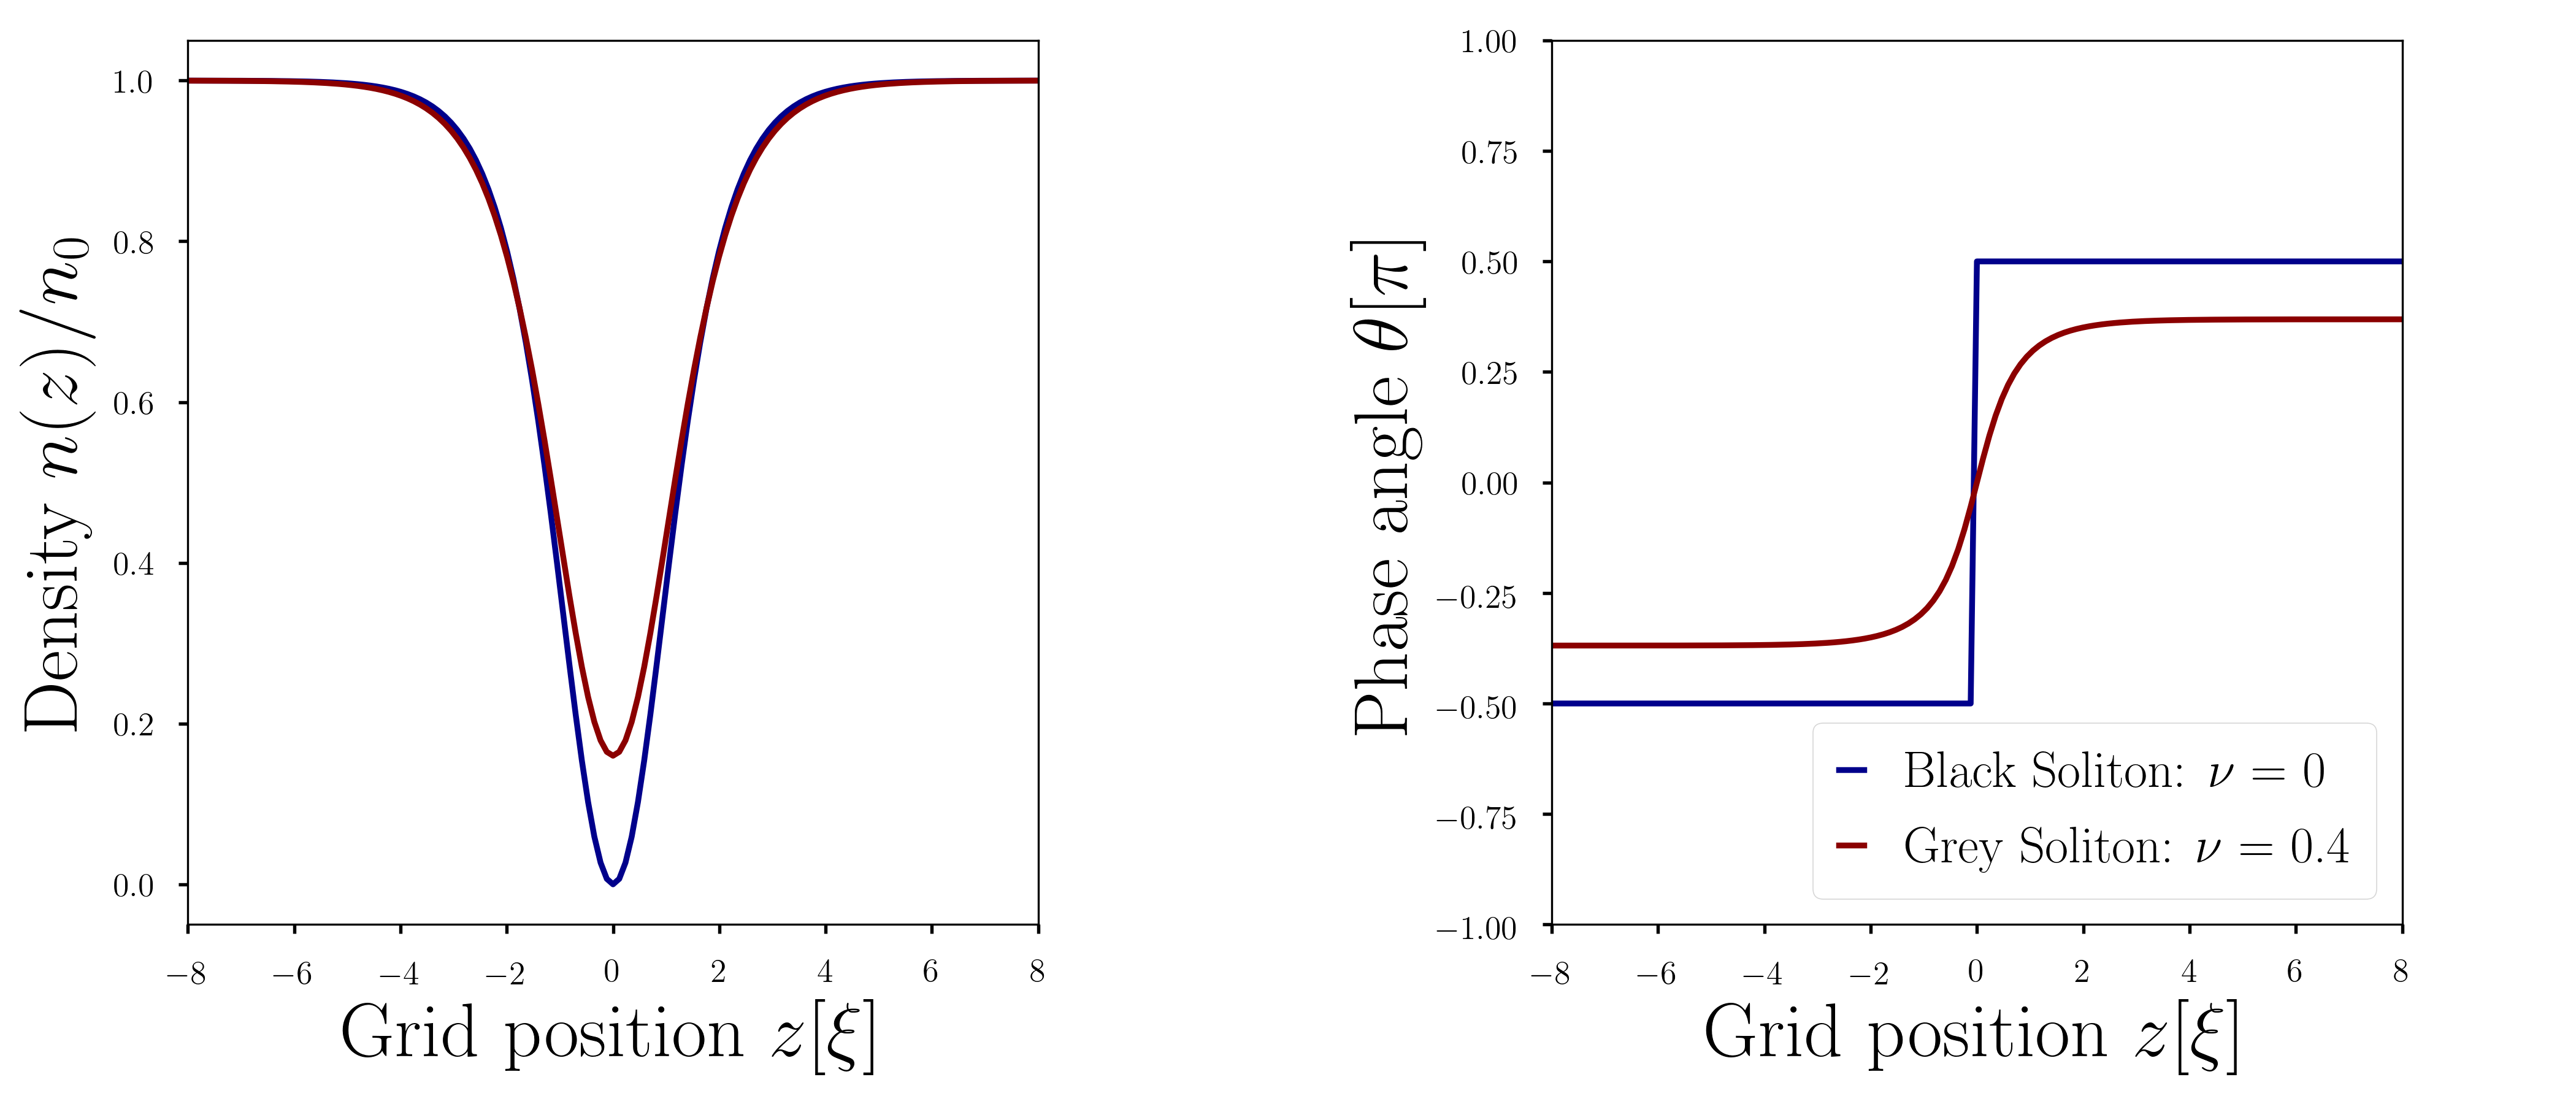
\includegraphics[scale = 0.35]{figures/black_and_grey}
\label{fig:SolitonAnalytical}
\caption{Density profile and phase of a single black and grey soliton}
\end{figure}

Solitons are localized density minima with a maximum density depression of $\sfrac{n_{\text{min}}}{n} = \nu^2$, \\ associated with a phase jump of $\Delta\theta \leq \pi$. They are called \textit{black}, if $v_s = 0$ and \textit{gray}, if $v_s \neq 0$. The physical momentum carried by the wave function due to the presence of the soliton  is given by 
\begin{align}
	p = m \int \dd z \ j(z) = -2\hbar n \nu \sqrt{1-\nu^2}
\end{align} 
with the current $j(z)$. It has a maximum at $\nu \approx 0.7 $\ \cite{Erne2012}.

\subsection{Vortices}
Another interesting excitation are vortices, which are a special property of superfluids. To get a better understanding of the density structure, we use cylindrical coordinates and evaluate the GPE for 
\begin{align}
	\psi(\mathbf{r}) = f(n, z)\operatorname{e}^{il\varphi}.
\end{align}
This results in an additional term, i.\,e. $ \sfrac{(\hbar l)^2}{2mn^2}$. which gives the kinetic energy resulting from its azimuthal velocity. The size of a typical vortex is about $\xi$. To visualize the density profile of a vortex we included a plot from \cite{ETH}.
\begin{figure}[H]
	\centering
	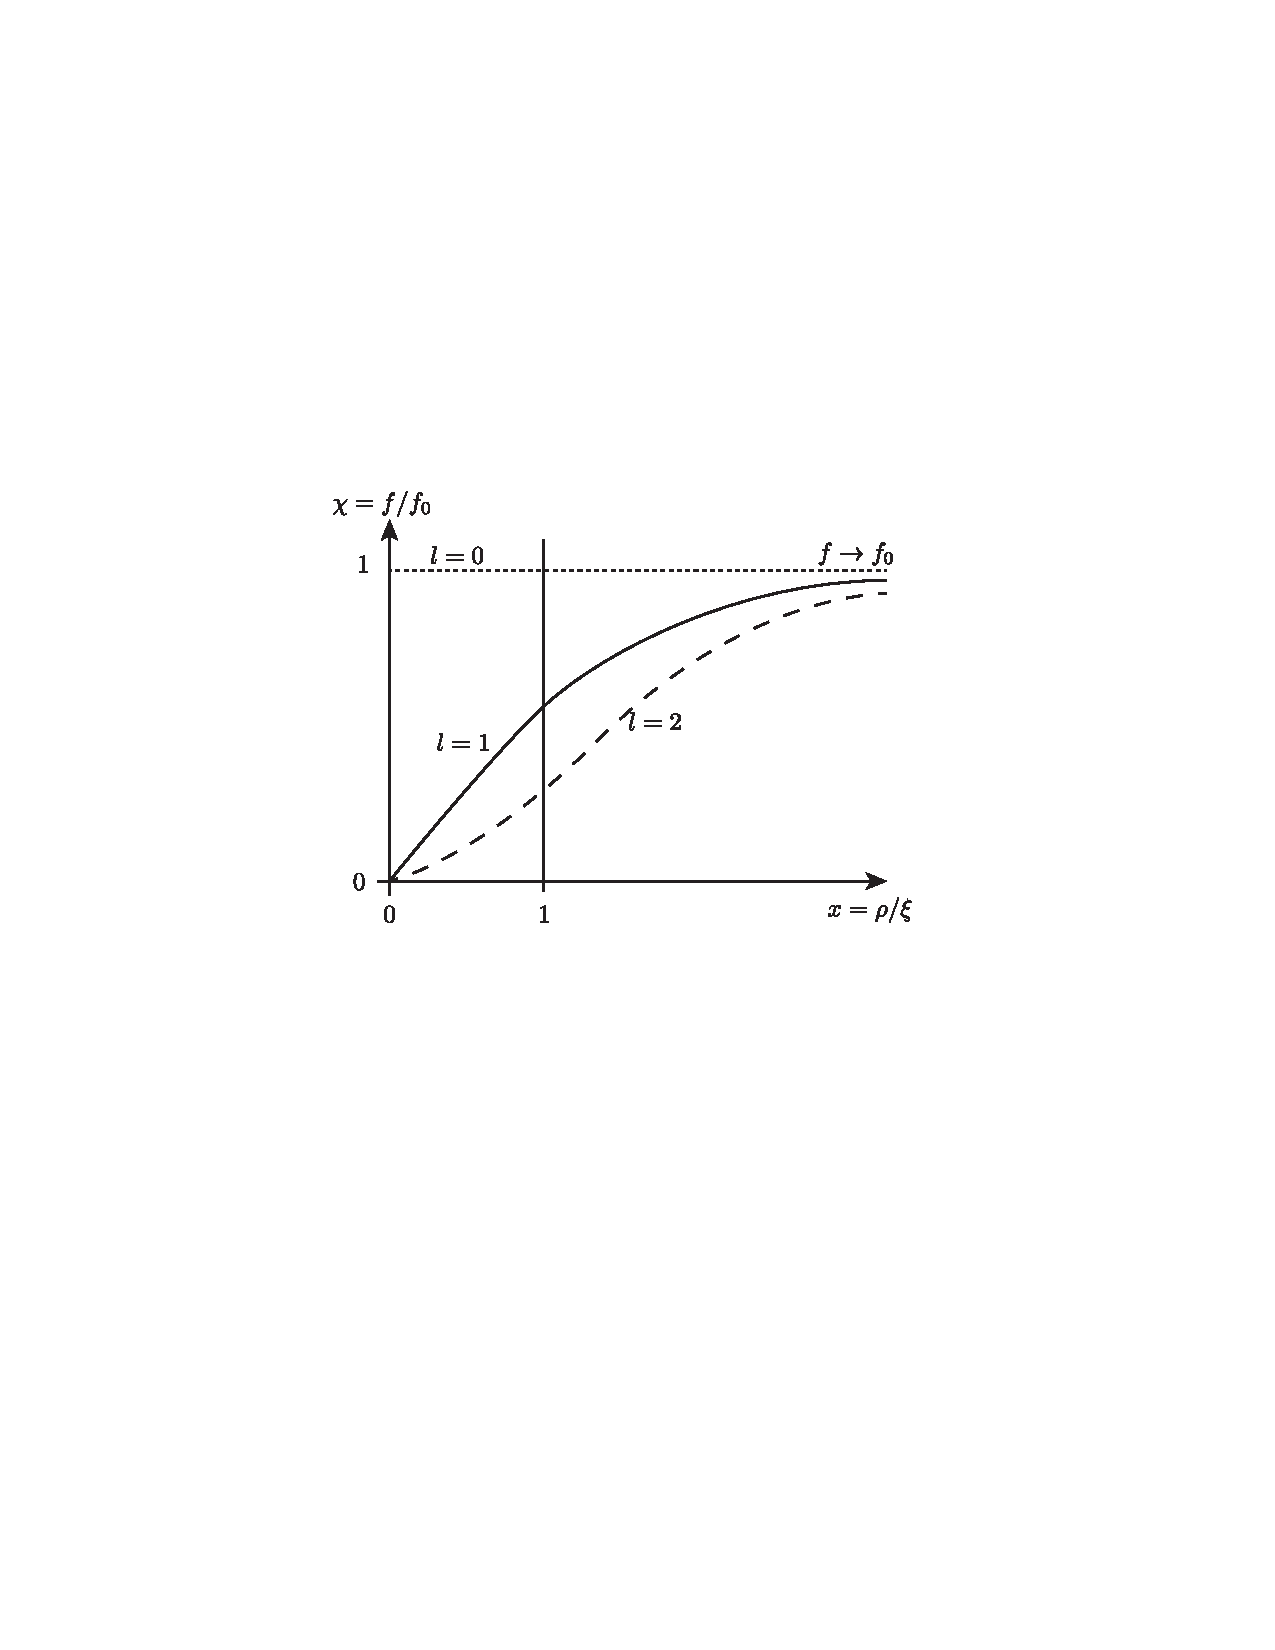
\includegraphics[scale = 0.6]{figures/vertex_density}
	\caption{Density profile of a vortex, taken from \cite{ETH} }
\end{figure}
Here, $\rho$ is the background density, $l = 1, 2$ \ is the charge of the vortex and $l=0$ \ is a situation without the presence of a vortex.

In this project, we are mainly interested in the evolution of different vortex constellations over time. This will be explained in more detail later on.

The final part of this introduction deals with the Split-Step Fourier method, our numerical approach for solving the GPE in this project.